\begin{figure}[p]
\centering
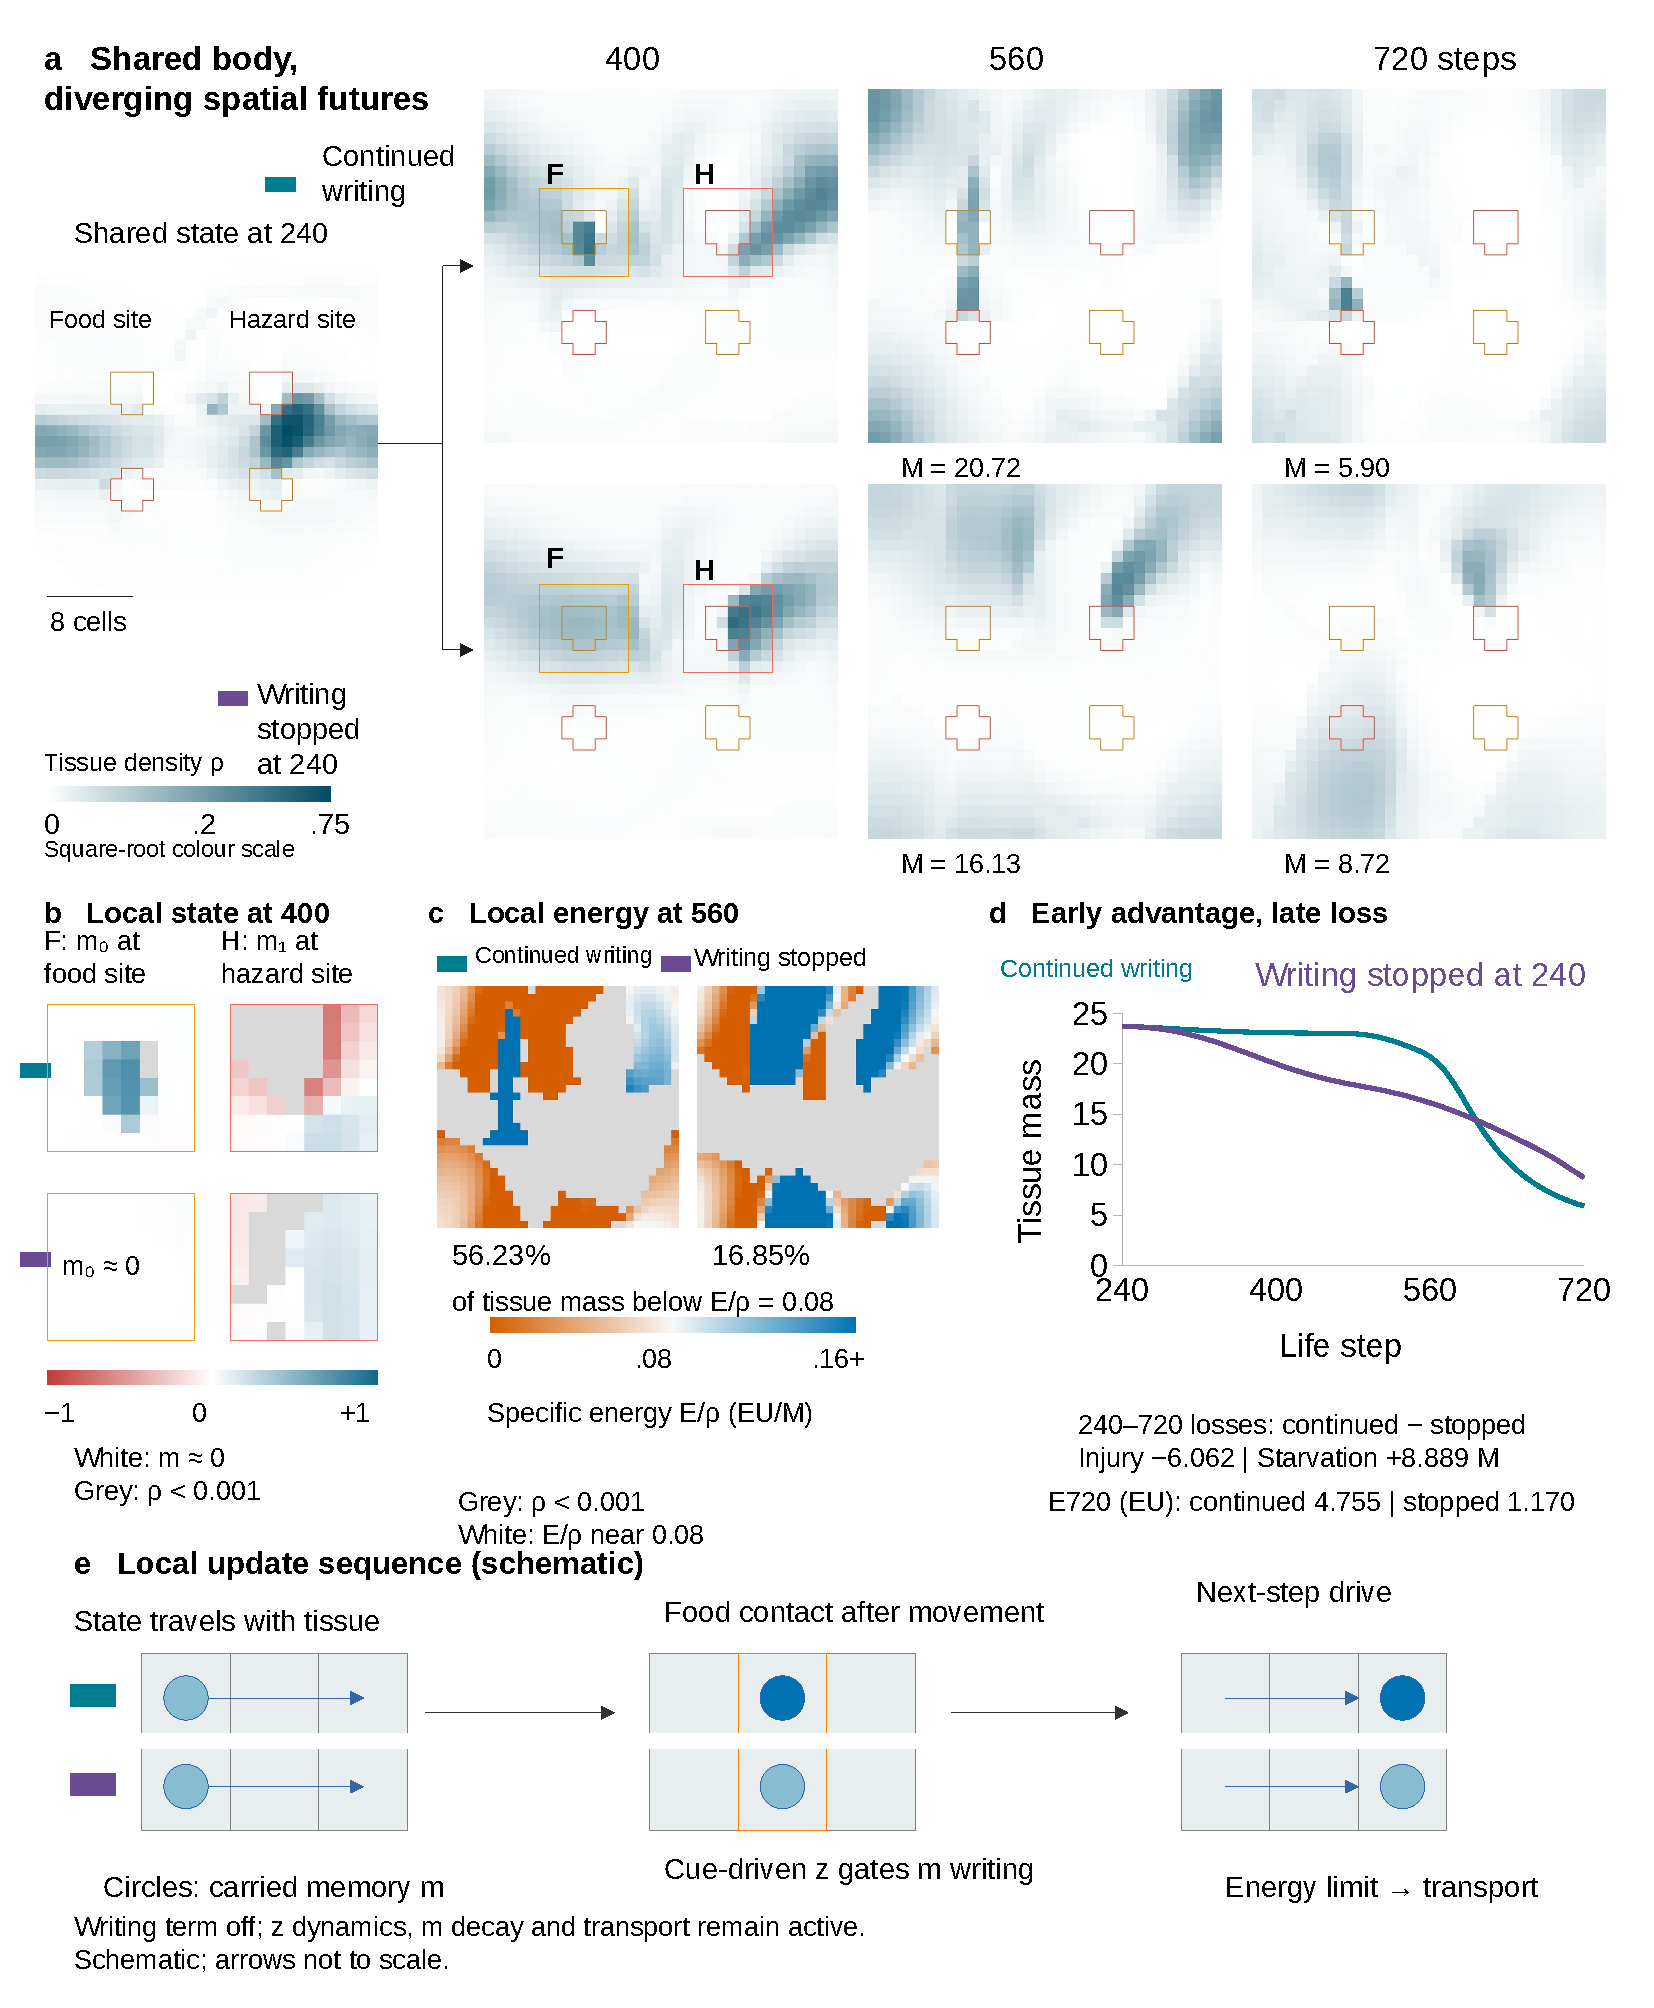
\includegraphics[width=0.90\linewidth]{figures/main/spatial_experience/spatial_state_divergence.pdf}
\caption{\textbf{Shared body, diverging spatial futures.}
\textbf{a,} The same complete acquired body and remaining world at step 240 continue with writing enabled (teal) or new writing stopped (purple). Density scenes at 400, 560 and 720 retain original periodic $32\times32$ coordinates and the same square-root colour scale. F/H mark Food/Hazard sites; F here is a food-site label, not the fuel F of Fig.~\ref{fig:allocation-feedback}. Scale bar, 8 cells.
\textbf{b,c,} Local $m_0/m_1$ at 400 and specific energy at 560 are observed fields, not isolated mediators. Grey masks $\rho<0.001$; low-energy percentages include all tissue mass.
\textbf{d,} The complete 61-point mass path shows early advantage followed by late loss; final energy has the opposite ordering.
\textbf{e,} Schematic of transport, cue-driven eligibility and writing, then subsequent energy-limited movement. Stopping new writing leaves $m$ decay, transport and eligibility active. This model has no tissue birth and is distinct from the generative models; the continued-writing future is reused.}
\label{fig:writing-turnover}
\end{figure}
